\documentclass[12pt, oneside, a4paper]{scrreprt}

\usepackage[manualmark,headsepline,footsepline]{scrlayer-scrpage}

\usepackage[german]{babel}
\usepackage[utf8]{inputenc}
\usepackage{graphicx} %Grafik aktivieren
\usepackage{float}
\usepackage[final]{pdfpages}
\usepackage{hyperref}
\usepackage{pdfcomment}
\usepackage{svg}

\usepackage{siunitx}  
\sisetup{locale = DE,separate-uncertainty}  

\usepackage[backend=biber]{biblatex}
\addbibresource{refs.bib}


%% used for pgfplots, tikzpicture
\usepackage{pgfplots}
\pgfplotsset{compat=newest}

%% the following commands are needed for some matlab2tikz features
\usetikzlibrary{plotmarks}
\usetikzlibrary{arrows.meta}
\usetikzlibrary{datavisualization}
\usetikzlibrary{datavisualization.formats.functions}
\usepgfplotslibrary{patchplots}
\usepackage{array}
\usepackage{grffile} 
\usepackage{amsmath}

\usepackage{todonotes}

\usepackage{listings}

\pgfplotsset{plot coordinates/math parser=false}
\newlength\fwidth

%%%%%%%%%%%%%%%%%%%%%%%%%%%%%%%%%%%%%%%%%%%%%%%%%%%%%%%%%%%%%%%%%%%%%%%%%%%%%%%%%%%%%%%%%%%%%%%%%%%%%%%%%%%%%%%%%%%%%%%%

%Kapitel-Layout
\usepackage{lmodern} 
\usepackage{xcolor}
\colorlet{chapter}{black!75}
\addtokomafont{chapter}{\color{chapter}}
\makeatletter% siehe De-TeX-FAQ
\renewcommand*{\chapterformat}{%
    \begingroup% damit \unitlength-Änderung lokal bleibt 
    \setlength{\unitlength}{1mm}% 
    \begin{picture}(20,20)(0,5)% 
    \setlength{\fboxsep}{0pt}% 
    \put(20,20){\line(1,0){\dimexpr 
    \textwidth-20\unitlength\relax\@gobble}}% 
    \put(0,0){\makebox(15,20)[r]{% 
    \fontsize{18\unitlength}{28\unitlength}\selectfont\thechapter 
    \kern-.04em% Ziffer in der Zeichenzelle nach rechts schieben 
    }}% 
    \end{picture} % <-- Leerzeichen ist hier beabsichtigt! 
    \newline
    \endgroup
}

\setlength\parindent{0pt}

%%%%%%%%%%%%%%%%%%%%%%%%%%%%%%%%%%%%%%%%%%%%%%%%%%%%%%%%%%%%%%%%%%%%%%%%%%%%%%%%%%%%%%%%%%%%%%%%%%%%%%%%%%%%%%%%%%%%%%%%

% Kopf- und Fußzeilen, Seitenränder etc.
% Kopf- und Fußzeilen ------------------------------------------------------
\pagestyle{scrheadings}

% Kopf- und Fußzeile auch auf Kapitelanfangsseiten -------------------------
\renewcommand*{\chapterpagestyle}{scrheadings}

% Schriftform der Kopfzeile ------------------------------------------------
\renewcommand{\headfont}{%
\normalfont
}

% Kopfzeile ----------------------------------------------------------------
\ihead{Regelungstechnisches Praktikum (RTP)}
\chead{}
\ohead{
\includegraphics[width=0.3\textwidth]{figure/oth-regensburg-logo}}
%
\setlength{\headheight}{21mm} % Höhe der Kopfzeile
%\setheadsepline[text]{0.4pt} % Trennlinie unter Kopfzeile

% Fußzeile -----------------------------------------------------------------
\ifoot{Name 1 Name 2}
\cfoot{\today}
\ofoot{\pagemark}


% erzeugt ein wenig mehr Platz hinter einem Punkt --------------------------
\frenchspacing 

\clubpenalty = 10000
\widowpenalty = 10000 
\displaywidowpenalty = 10000


\newcommand{\mt}[1]{\textrm{#1}}



%%%%%%%%%%%%%%%%%%%%%%%%%%%%%%%%%%%%%%%%%%%%%%%%%%%%%%%%%%%%%%%%%%%%%%%%%%%%%%%%%%%%%%%%%%%%%%%%%%%%%%%%%%%%%%%%%%%%%%%%
%%%%%%%%%%%%%%%%%%%%%%%%%%%%%%%%%%%%%%%%%%%%%%%%%%%%%%%%%%%%%%%%%%%%%%%%%%%%%%%%%%%%%%%%%%%%%%%%%%%%%%%%%%%%%%%%%%%%%%%%
%%%%%%%%%%%%%%%%%%%%%%%%%%%%%%%%%%%%%%%%%%%%%%%%%%%%%%%%%%%%%%%%%%%%%%%%%%%%%%%%%%%%%%%%%%%%%%%%%%%%%%%%%%%%%%%%%%%%%%%%

\begin{document}

    \begin{titlepage}

        \begin{tabular}{l r} 
    
        
\includegraphics[width=0.4\textwidth]{../03_RTP-Ausarbeitung_Beispiel_TeX/Bilder/oth-regensburg-logo.jpg}
        &
            
    \end{tabular}


    \begin{minipage} [c] [8.5cm] [b] {\textwidth}
        \Huge{
            \begin{center}
                \textbf{Praktikum Regelungstechnik (RTP)}\\[0.8cm]
                \textbf{Versuch T2: Systemidentifikation} \\[1.5cm]
                \par
                {\large Versuch 1}\\[1cm]
                %{\large empty} \\[1cm]
            \end{center}
            }
        
    \end{minipage}

    \vspace{0.1cm}

        
    \begin{minipage} [c] [3.5cm] [b] {\textwidth}
        \begin{center}
        \vspace{0.3cm}
        Gruppe 38\\
        Marius Off\\
        Janis Graf\\
        \vspace{0.5cm}
        \texttt{Dokument-Version: 02}\\
        \end{center}
    
    \end{minipage}


    \end{titlepage}

    \tableofcontents


    \chapter{Preperations}\label{chap:preperations}
    
    In preparation for this experiment, the files provided in ELO were downloaded and saved \cite{RTP_Experiments}. In addition, the step responses for various system behaviours were researched. As tasked in Tasks $task:a)V$ and $task:b)V$ $task:c)V$ $task:d)V$ \\
        
        \section{Different basic system behaviors}
        \todo{Check names of coloumns again}
        
            \begin{tabular}{m{4.5cm} m{6.5cm} >{\centering\arraybackslash}m{3.5cm}}
                \textbf{Systemverhalten}                           & \textbf{Übertragungsfunktion}                                                                                                                    & \textbf{Visualization}                                      \\
                \hline
                {P-Glied ($K_p$)}                                  & $G(s) = K_p \refstepcounter{equation}(\theequation)\label{eq:P}$                                                                          & \resizebox{2cm}{2cm}{% placeholder for P-Glied


\tikz \datavisualization
    [scientific axes={clean, standard labels},
    visualize as smooth line,
    x axis={label=$t$, ticks=none},
    y axis={label=$h(t)$, ticks=none}]
    data [format=function] {
    var x : interval [-1:5] samples 100;
    func y = (\value x > 0) ? 2 : 0;
};

} \\[4pt]
                {PT$_1$-Glied ($K_p$, $T_1$)}                      & $G(s) = \dfrac{K_p}{T_1 s + 1} \refstepcounter{equation}(\theequation)\label{eq:PT1}$                                                     & \resizebox{2cm}{2cm}{% placeholder for PT1-Glied


\tikz \datavisualization
    [scientific axes={clean, standard labels},
    visualize as smooth line,
    x axis={label=$t$, ticks=none},
    y axis={label=$h(t)$, ticks=none}]
    data [format=function] {
    var x : interval [0:10] samples 50;
    func y = 1 - exp(-\value x / 2);
};

} \\[4pt]
                {PT$_2$-Glied ($K_p$, $\omega_0$, $D$)}            & $G(s) = \dfrac{K_p}{\frac{1}{\omega_0^{2}} s^{2} + \frac{2D}{\omega_0} s + 1} \refstepcounter{equation}(\theequation)\label{eq:PT2_w0_D}$ & \resizebox{2cm}{2cm}{% placeholder for PT2-Glied


\tikz \datavisualization
    [scientific axes={clean, standard labels},
    visualize as smooth line,
    x axis={label=$t$, ticks=none},
    y axis={label=$h(t)$, ticks=none}]
    data [format=function] {
    var x : interval [0:20] samples 100;
    func y = 1 - exp(-0.2 * \value x) * (cos(deg(0.9798 * \value x)) + (0.2/0.9798) * sin(deg(0.9798 * \value x)));
};

} \\[4pt]
                {PT$_2$-Glied für $D \ge 1$ ($K_p$, $T_1$, $T_2$)} & $G(s) = \dfrac{K_p}{(T_1 s + 1)(T_2 s + 1)} \refstepcounter{equation}(\theequation)\label{eq:PT2_T1_T2}$                                  & \resizebox{2cm}{2cm}{% placeholder for PT2-Glied (D>=1)


\tikz \datavisualization
    [scientific axes={clean, standard labels},
    visualize as smooth line,
    x axis={label=$t$, ticks=none},
    y axis={label=$h(t)$, ticks=none}]
    data [format=function] {
    var x : interval [0:10] samples 50;
    func y = 1 - (2*exp(-\value x/2) - exp(-\value x));
};

} \\[4pt]
                {I-Glied ($K_I$)}                                  & $G(s) = \dfrac{K_I}{s} \refstepcounter{equation}(\theequation)\label{eq:I}$                                                               & \resizebox{2cm}{2cm}{% placeholder for I-Glied


\tikz \datavisualization
    [scientific axes={clean, standard labels},
    visualize as smooth line,
    x axis={label=$t$, ticks=none},
    y axis={label=$h(t)$, ticks=none}]
    data [format=function] {
    var x : interval [0:10] samples 10;
    func y = 0.5 * \value x;
};

} \\[4pt]
                {IT$_1$-Glied ($K_I$, $T_1$)}                      & $G(s) = \dfrac{K_I}{s (T_1 s + 1)} \refstepcounter{equation}(\theequation)\label{eq:IT1}$                                                 & \resizebox{2cm}{2cm}{% placeholder for IT1-Glied


\tikz \datavisualization
    [scientific axes={clean, standard labels},
    visualize as smooth line,
    x axis={label=$t$, ticks=none},
    y axis={label=$h(t)$, ticks=none}]
    data [format=function] {
    var x : interval [0:10] samples 50;
    func y = 0.5 * (\value x - 2 + 2*exp(-\value x/2));
};

} \\[4pt]
                {D-Glied ($K_D$)}                                  & $G(s) = K_D\, s \refstepcounter{equation}(\theequation)\label{eq:D}$                                                                      & \resizebox{2cm}{2cm}{% placeholder for D-Glied


\tikz \datavisualization
    [scientific axes={clean, standard labels},
    visualize as smooth line,
    x axis={label=$t$, ticks=none},
    y axis={label=$h(t)$, ticks=none}]
    data [format=function] {
    var x : interval [0:5] samples 50;
    func y = (\value x < 0.1) ? 10 : 0;
};

} \\[4pt]
                {DT$_1$-Glied ($K_D$, $T_1$)}                      & $G(s) = \dfrac{K_D\, s}{T_1 s + 1} \refstepcounter{equation}(\theequation)\label{eq:DT1}$                                                 & \resizebox{2cm}{2cm}{% placeholder for DT1-Glied


\tikz \datavisualization
    [scientific axes={clean, standard labels},
    visualize as smooth line,
    x axis={label=$t$, ticks=none},
    y axis={label=$h(t)$, ticks=none}]
    data [format=function] {
    var x : interval [0:10] samples 50;
    func y = exp(-\value x);
};

} \\[4pt]
                {T$_t$-Glied ($K_p$, $T_t$)}                       & $G(s) = K_p\, e^{-T_t s} \refstepcounter{equation}(\theequation)\label{eq:Tt}$                                                            & \resizebox{2cm}{2cm}{% placeholder for Tt-Glied


\tikz \datavisualization
    [scientific axes={clean, standard labels},
    visualize as smooth line,
    x axis={label=$t$, ticks=none},
    y axis={label=$h(t)$, ticks=none}]
    data [format=function] {
    var x : interval [0:10] samples 50;
    func y = (\value x > 2) ? 1 : 0;
};

} \\
            \end{tabular}
        
            \cleardoublepage

            \subsection{P-Glied}

                \subsubsection{Explanation}
                \todo[inline]{Check explanation of the P-Glied again, look into script}

                    Proportional-Glied, show a constant behavior in steady state for a constant input. The output is directly proportional to the input, with the proportionality constant being $K_p$.
                    The equation for a P-Glied is given by 
                    \begin{equation}
                        x_a(t) = K_p x_e(t)
                    \end{equation}
                    where $x_a(t)$ is the output and $x_e(t)$ is the input. The transfer function of a P-Glied is $G(s) = K_p$ \ref{eq:P}.

                    \missingfigure{Missing figure for the P-Glied}
                \subsubsection{Parameters needed for characterization}
                    The only parameter needed to characterize a P-Glied is the proportional gain $K_p$. This parameter determines the steady-state gain of the system and how much the output will change in response to a change in the input.

                \subsubsection{Step and Impulse response}
                    The step response of a P-Glied is a step function that reaches a steady state value of $K_p$ times the input step magnitude. The impulse response is an impulse function scaled by $K_p$.

                    \missingfigure{Missing figure for the P-Glied step and impulse response}

            \cleardoublepage

            \subsection{PT$_1$-Glied}

                \subsubsection{Explanation}
                \todo[inline]{Check explanation of the PT1-Glied again, look into script}
                    The PT$_1$-Glied is a first-order delay system that consists of a proportional element and a first-order part. The transfer function of a PT$_1$-Glied is given by 
                    \begin{equation}
                    T_1 \dot{x}_a + x_a(t) = K_p x_e(t)
                    \end{equation}
                    or equation \ref{eq:PT1}, where $K_p$ is the proportional gain and the final value of the function and $T_1$ is the time constant. 
                
                    \missingfigure{Missing figure for the PT$_1$-Glied}

                \subsubsection{Parameters needed for characterization}
                    For the characterization of a PT$_1$-Glied, the parameters needed are the proportional gain $K_p$ and the time constant $T_1$. The proportional gain $K_p$ determines the steady-state gain of the system, while the time constant $T_1$ determines how quickly the system responds to changes in the input.
                    The System is also characterized by its initial tangent, which is given by $y(t) = \frac{K_p}{T_1} t$. The point at which the initial tangent intersects the steady state value of the step response can be used to determine the time constant $T_1$. $T_1$ is the time it takes for the system to reach approximately $63\%$ of its final value in response to a step input. The threefold multiple of the time constant $T_1$ at which the system reaches $95\%$ of its final value can also be used to characterize the system's response speed. 

                \subsubsection{Step and Impulse response}
                    The step response of a PT$_1$-Glied is an exponential function that approaches a steady state value of $K_p$ times the input step magnitude, with a time constant of $T_1$. The impulse response is an exponential function scaled by $K_p/T_1$.

            \cleardoublepage

            \subsection{PT$_2$-Glied}

                \subsubsection{Explanation}
                \todo[inline]{Check explanation of the PT2-Glied again, look into script}
                    
                    A PT$_2$-Glied is a second-order delay system that consists of a proportional element and a second-order part, which appares delayed and oscillatory behavior becuase of its second order differential nature. The transfer function of a PT$_2$-Glied is given by 
                    \begin{equation}
                        \frac{1}{\omega_0^2} \ddot{x}_a + \frac{2D}{\omega_0} \dot{x}_a + x_a(t) = K_p x_e(t)
                    \end{equation}
                    or equation \ref{eq:PT2_w0_D} , where $K_p$ is the proportional gain, $\omega_0$ is the natural frequency, and $D$ is the damping ratio.

                    \missingfigure{Missing figure for the PT$_2$-Glied}

                \subsubsection{Parameters needed for characterization}
                    For the characterization of a PT$_2$-Glied, the parameters needed are the proportional gain $K_p$, the natural frequency $\omega_0$, and the damping ratio $D$. The proportional gain $K_p$ determines the steady-state gain of the system, while the natural frequency $\omega_0$ and damping ratio $D$ determine the oscillatory behavior and response speed of the system. The damping ratio $D$ indicates whether the system is underdamped ($D < 1$), critically damped ($D = 1$), overdamped ($D > 1$) or undamped ($D = 0$).

                    For an underdamped system ($D < 1$), the step response will exhibit oscillations before settling to the steady state value. The natural frequency $\omega_0$ determines the frequency of these oscillations, while the damping ratio $D$ determines how quickly the oscillations decay. 
                    For a critically damped system ($D = 1$), the step response will reach the steady state value without oscillating, and it will do so as quickly as possible without overshooting. It is often reached by putting two PT$_1$-Glied in series, which results in the transfer function given by 
                    \begin{equation}
                        T_1T_2 \ddot{x}_a + (T_1 + T_2) \dot{x}_a + x_a(t) = K_p x_e(t)
                    \end{equation}
                    or 
                    \begin{equation}
                        h(t) = K_P \left(1 - (1 + \omega_0 t)e^{-\omega_0 t}\right)
                    \end{equation}
                    For an overdamped system ($D > 1$), the step response will reach the steady state value without oscillating, but it will take longer to do so than a critically damped system. The Transfer function can be rewritten as 
                    \begin{equation}
                        h(t) = K_p \left(1 + \frac{1}{\lambda_1 - \lambda_2}(\lambda_2e^{-\lambda_1t} - \lambda_1e^{-\lambda_2t})\right)
                    \end{equation} 
                    where $\lambda_1$ and $\lambda_2$ are the eigenvalues of the characteristic equation of the system, given by 
                    \begin{equation}
                        \lambda_{1,2} = -D\omega_0 \pm \omega_0\sqrt{D^2 - 1}
                    \end{equation}    
                    The time constants of the system can be determined from these roots, and they indicate how quickly the system responds to changes in the input.
                    For an undamped system ($D = 0$), the step response will exhibit sustained oscillations at the natural frequency $\omega_0$.

                    For the case $0 < D < 1$, the transfer function can be rewritten as 
                    \begin{equation}
                        h(t) = K_p \left(1 - \frac{e^{-\omega_0 D t}}{\sqrt{1 - D^2}} \sin(\omega_d t + \phi)\right)
                    \end{equation}

                    The Periodic time of the oscillations can be determined from the damped natural frequency 
                    \begin{equation}
                        T_d = \frac{2\pi}{\omega_d} = \frac{2\pi}{\omega_0 \sqrt{1 - D^2}}
                    \end{equation}
                    The Transferfunction can be caracterized by the upper and lower envelope of the oscillations, which are given by 
                    \begin{equation}
                        h^\pm(t) = K_p (1 \pm \frac{e^-D\omega_0 t}{\sqrt{1-D^2}})
                    \end{equation}
                    
                    The over swing time $t_{max}$, which is the time at which the first maximum of the step response occurs, can be determined from the equation 

                    \begin{equation}
                        t_{max} = \frac{\pi}{\omega_d} = \frac{\pi}{\omega_0 \sqrt{1 - D^2}}
                    \end{equation}

                    The overshoot $h_{max}$, can be determined from the equation 
                    \begin{equation}
                        h_{max} = h(t_{max}) = K_p \left(1 + e^{-\pi D/\sqrt{1-D^2}}\right)
                    \end{equation}
                    The normalized overshoot value $\ddot{u}$ can be determined from the equation
                    \begin{equation}
                        \ddot{u} = \frac{h_{max} - h(\infty)}{h(\infty)} = e^{\frac{-\pi D}{\sqrt{1-D^2}}}
                    \end{equation}
                    which can be used to determine the damping ratio $D$ from the overshoot of the step response. Given by the equation 
                    \begin{equation}
                        D = \frac{\left| \ln(\ddot{u}) \right|}{\sqrt{\pi^2 + \ln^2(\ddot{u})}}
                    \end{equation}


                \subsubsection{Step and Impulse response}

            \cleardoublepage
            
            \subsection{I-Glied}
                \subsubsection{Explanation}

                    Integral-Glied, are transfer functions that consist of an integrator of input signal, the output $x_a(t)$ is proportional to the integral of the input $x_e(t)$, with the proportionality constant being $K_I$. The transfer function of an I-Glied is given by $G(s) = \frac{K_I}{s}$ \ref{eq:I}. given by the equation
                    \begin{equation}
                        x_a(t) = K_I \int_0^t x_e(\tau) d\tau
                    \end{equation}
                    Equation \ref{eq:I} can also be rewritten as
                    \begin{equation}                    
                        h(t) = K_I \int_0^t \sigma(\tau) d\tau = K_I t
                    \end{equation} 

                    \missingfigure{Missing figure for the I-Glied}
                

                \subsubsection{Parameters needed for characterization}
                    The only parameter needed to characterize an I-Glied is the integral gain $K_I$. This parameter determines how quickly the output will change in response to a change in the input. The step response of an I-Glied is a ramp function that increases linearly with time, with a slope of $K_I$ times the input step magnitude. The impulse response is a step function scaled by $K_I$.

                \subsubsection{Step and Impulse response}
                    The step response of an I-Glied is a ramp function that increases linearly with time, with a slope of $K_I$ times the input step magnitude. The impulse response is a step function scaled by $K_I$.

            \cleardoublepage

            \subsection{IT$_1$-Glied}
                \subsubsection{Explanation}
                    The IT$_1$-Glied is a system that consists of an integrator and a first-order part. The transfer function of an IT$_1$-Glied is given by $G(s) = \frac{K_I}{s (T_1 s + 1)}$ \ref{eq:IT1}, where $K_I$ is the integral gain and $T_1$ is the time constant. It could be seen as a combination of an I-Glied and a PT$_1$-Glied. The transfer function can be rewritten as
                    \begin{equation}
                        h(t) = K_I \left[t-T_1({1-\exp^{-\frac{t}{T_1}}})\right]
                    \end{equation} 

                    \missingfigure{Missing figure for the IT$_1$-Glied}

                \subsubsection{Parameters needed for characterization}
                    For the characterization of an IT$_1$-Glied, the parameters needed are the integral gain $K_I$ and the time constant $T_1$. The integral gain $K_I$ determines proportionality of the function to the integral of the input, while the time constant $T_1$ determines how delayed the response of the system is to changes in the input.

                \subsubsection{Step and Impulse response}
                    The step response of an IT$_1$-Glied is a function that increases with time, with a shape that is determined by the integral gain $K_I$ and the delay caused by the time constant $T_1$. The impulse response is a function that slowly (with a delay and a shape determined by $T_1$) increases from zero to a the value of the integral of the input impulse scaled by $K_I$.

                    \missingfigure{Missing figure for the IT$_1$-Glied step and impulse response}

            \cleardoublepage

            % \subsection{D-Glied}
                
            %     \subsubsection{Explanation}

            %     \subsubsection{Parameters needed for characterization}

            %     \subsubsection{Step and Impulse response}

            % \cleardoublepage
                
            % \subsection{DT$_1$-Glied}

            %     \subsubsection{Explanation}

            %     \subsubsection{Parameters needed for characterization}

            %     \subsubsection{Step and Impulse response}

            % \cleardoublepage

            % \subsection{T$_t$-Glied}
                
            %     \subsubsection{Explanation}

            %     \subsubsection{Parameters needed for characterization}

            %     \subsubsection{Step and Impulse response}

            \cleardoublepage

        


    \chapter{Experiment T2: System identification}

        For the 3 systems investigated in this experiment, the following paragraphs will present the experimentally identified system parameters, a documentation of the results, a real-world example of such a system, and a comparison of the given system with the ideal response of the identified system. The identifided systems are a PT1-glied for system 0 with a step-function input\ref{sec:system0-pt1}, a PT2-glied for system 1 with a Dirac-impulse input\ref{sec:system1-pt2}, and an IT1-glied for system 2 with a step-function input\ref{sec:system2-it1}.

        \section{System 0 --- PT1}\label{sec:system0-pt1}
            
            \subsection{Experimentaly Identified system parameters}
                    The experimentally identified parameters for the PT1 system are as follows:
                    \begin{itemize}
                        \item Proportional gain $K_p$: [add value]
                        \item Time constant $T_1$: [add value]
                    \end{itemize}

            \begin{figure}[ht]
                \centering
                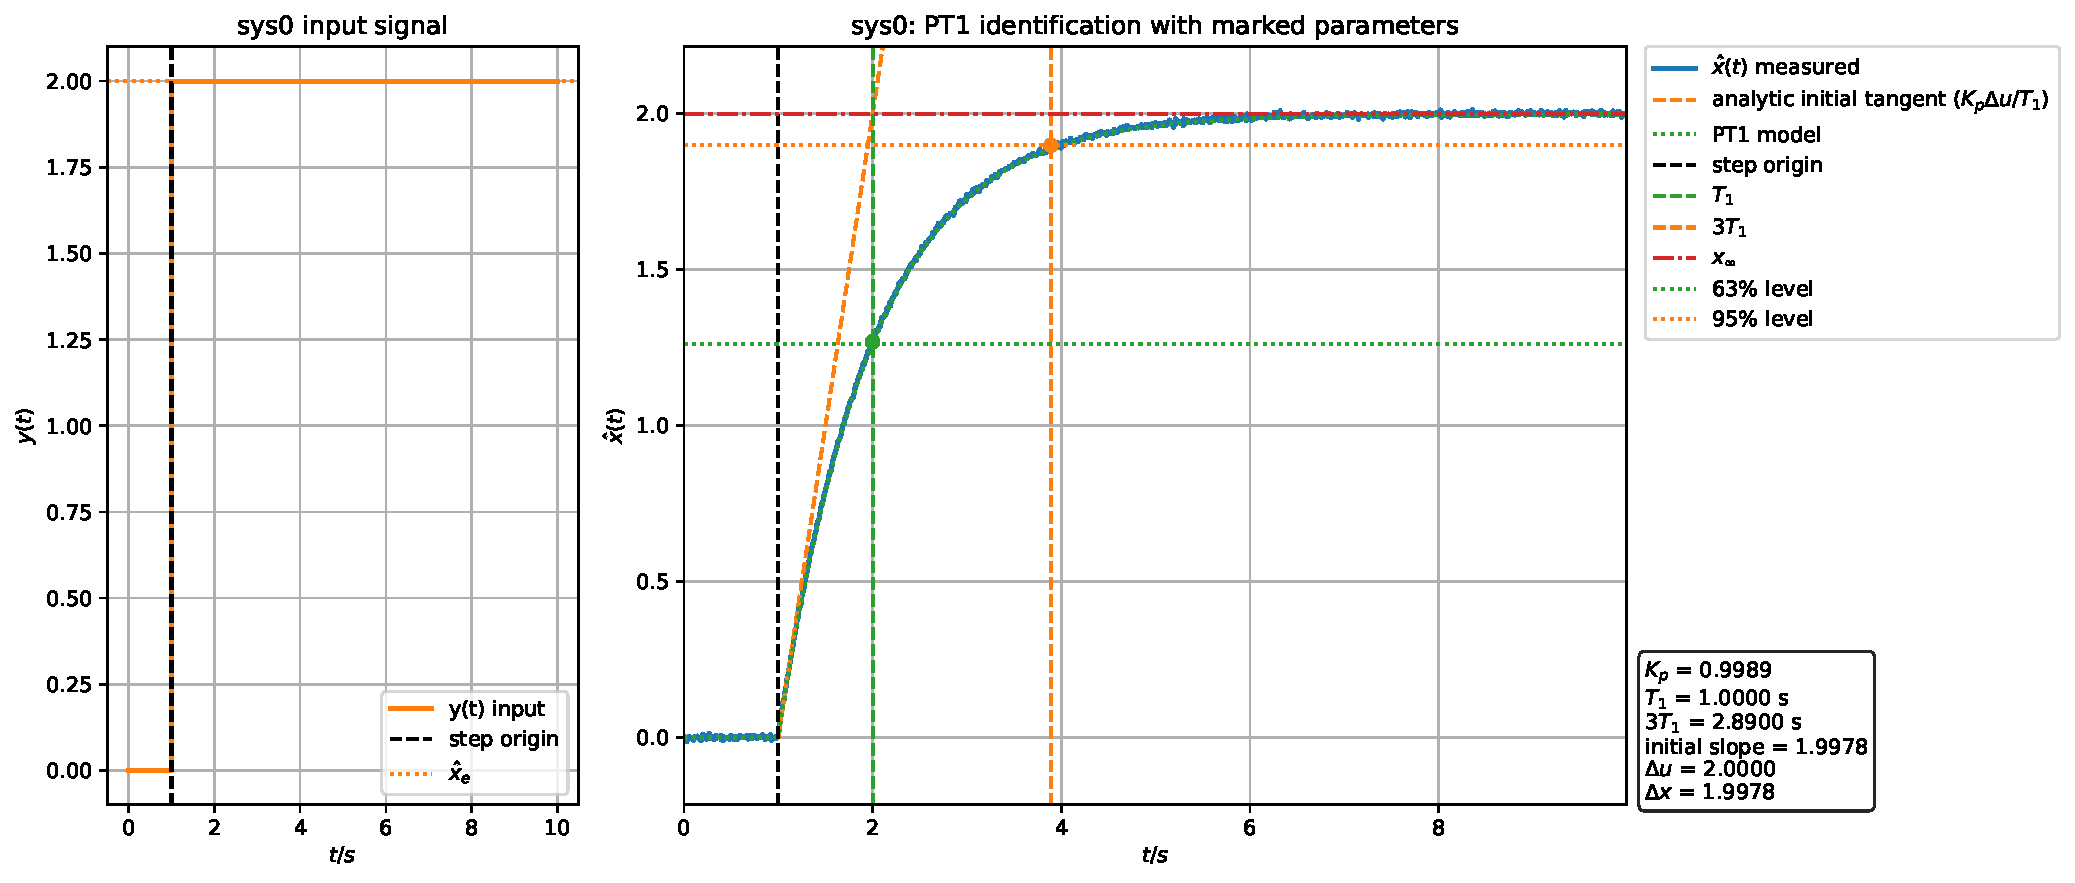
\includegraphics[width=0.8\textwidth]{../02_Preperations/figure_out/sys0_pt1_identification.pdf}
                \caption[]{}
            \end{figure}

            \todo[inline]{add parameters}

            \subsection{Documentation of the results}

                \subsubsection{Essential Commands}

                \todo[inline]{add essential commands for PT1 identification}

                \subsubsection{Differential Equation}

                \todo[inline]{add differential equation for PT1 system}

                \subsubsection{Transfer Function}

                \todo[inline]{add transfer function for PT1 system}

            \subsection{Realworld Example}

                A practical example of such a PT1 system with impulsive excitation is the temperature response of a small metal body to a brief heat flux. If, for example, a metal rod is briefly excited by a heat source (e.g. hot air or a laser) --- comparable to a Dirac impulse --- the body heats up abruptly and then cools down again via heat conduction and dissipation to the surroundings. The thermal behaviour follows a PT1 model: the temperature rises briefly due to the pulse (corresponding to the step in the output signal) and then falls back to the original level exponentially with a characteristic time constant. The time constant depends on the material properties (heat capacity, thermal conductivity) and the environmental conditions (e.g. convection, radiation). Such system responses frequently occur in sensor technology, materials analysis or in the case of short control pulses in electronic or thermal systems.description of the respective input and output variables.

            \subsection{Comparison of given System with the response of the identified system}

            \todo[inline]{add short text about differences of the ideal system to the messured PT1 system}

        
            \begin{figure}[ht]
                \centering
                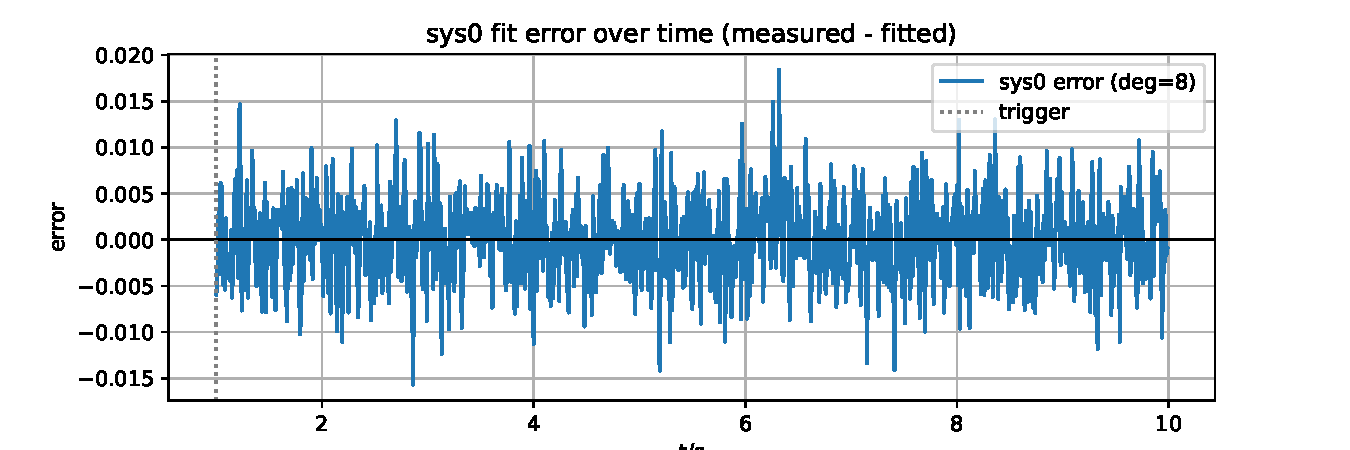
\includegraphics[width=0.8\textwidth]{../02_Preperations/figure_out/sys0_polyfit_error.pdf}
                \caption[]{}
            \end{figure}


                \subsubsection{Deviations of the System}

        \cleardoublepage

        \section{System 1}\label{sec:system1-pt2}

            System 1 is a PT2 system, reacting to a Dirac impulse input and showing a damped oscillatory behaviour ($0 < D < 1$).
            
            \subsection{Experimentaly Identified system parameters}

                The experimentally identified parameters for the PT2 system are as follows:
                \begin{itemize}
                    \item overshoot $h_{max}$: [add value]
                    \item over swing time $t_{max}$: [add value]
                    \item the damping ratio $D$: [add value]
                    \item the natural frequency $\omega_0$: [add value]
                    \item the periodic time of the oscillations $T_d$: [add value]
                \end{itemize}

            
            \todo[inline]{add parameters}
            
            \begin{figure}[ht]
                \centering
                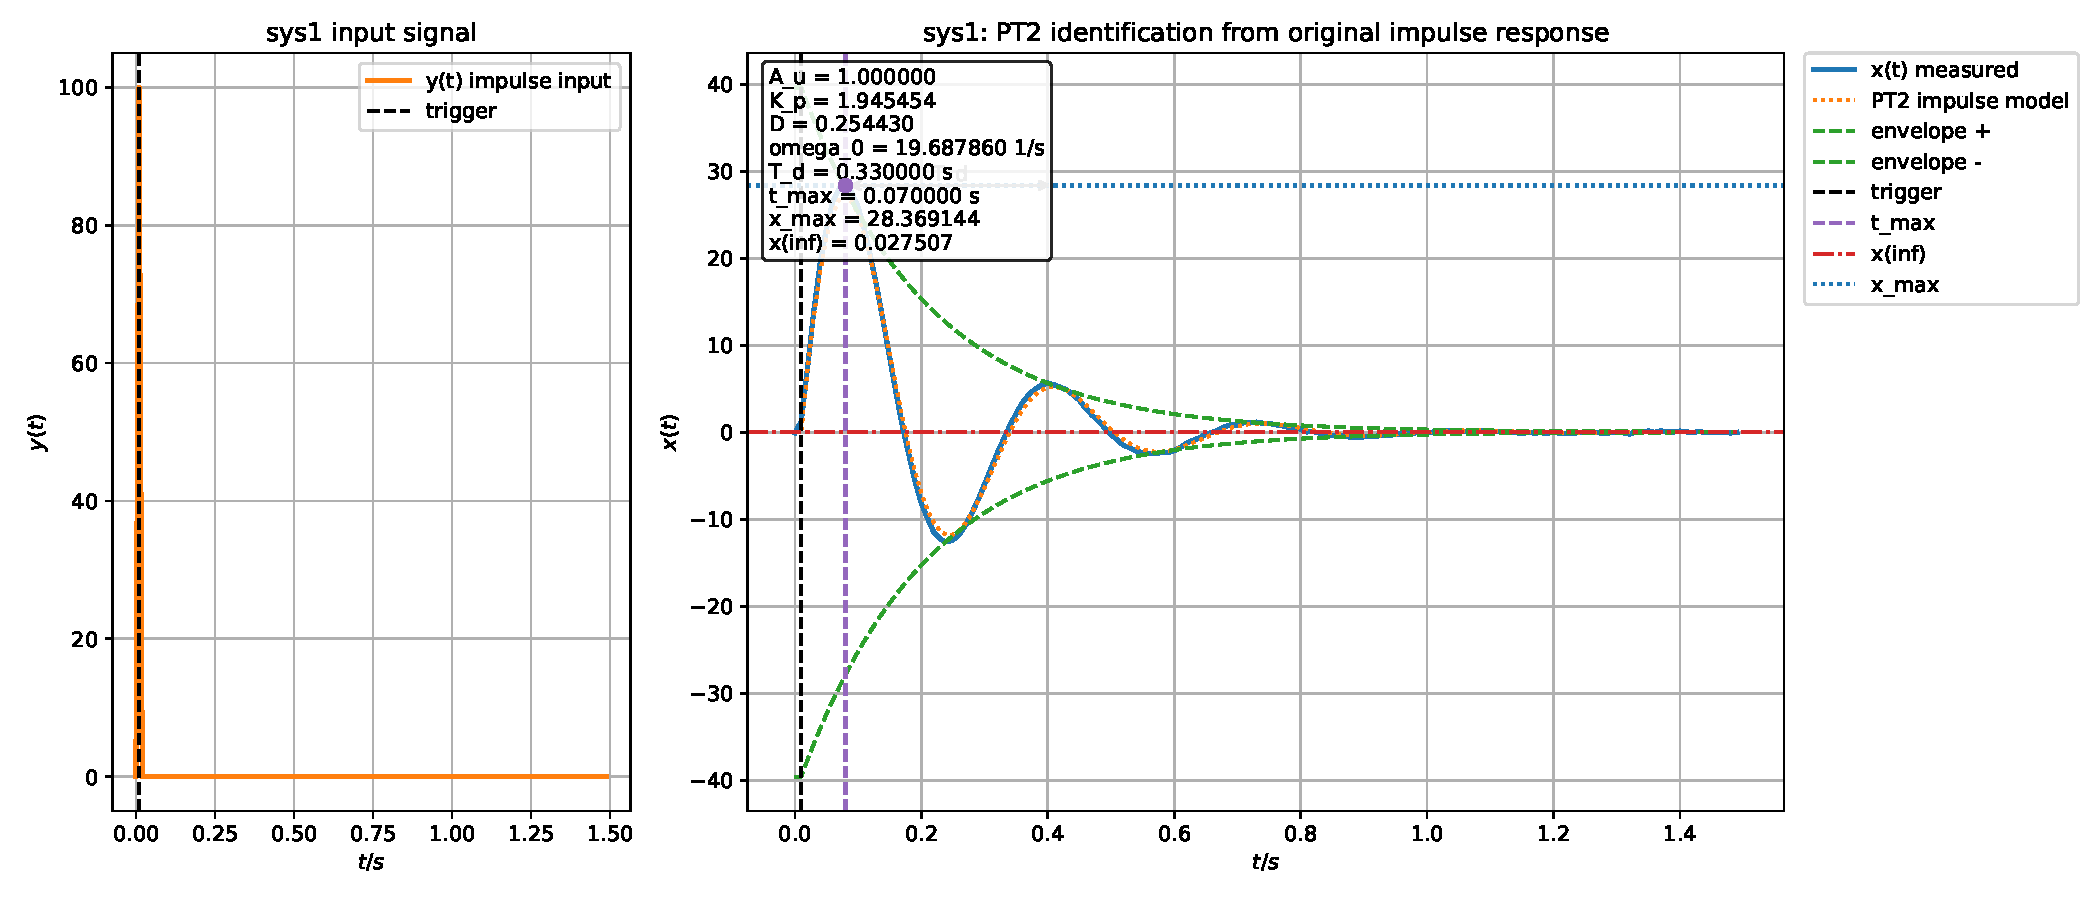
\includegraphics[width=0.8\textwidth]{../02_Preperations/figure_out/sys1_pt2_identification.pdf}
                \caption[]{}
            \end{figure}

            \subsection{Documentation of the results}

                \subsubsection{Essential Commands}
                
                \todo[inline]{add essential commands for PT2 identification}

                \subsubsection{Differential Equation}

                \todo[inline]{add differential equation for PT2 system}

                \subsubsection{Transfer Function}

                \todo[inline]{add transfer function for PT2 system}

            \subsection{Realworld Example}

                \todo[inline]{add realworld example for PT2 system, look into script}
                description of the respective input and output variables.

            \subsection{Comparison of given System with the response of the identified system}
            
                \todo[inline]{add short text about differences of the ideal system to the messured PT2 system}

                \begin{figure}[ht]
                    \centering
                    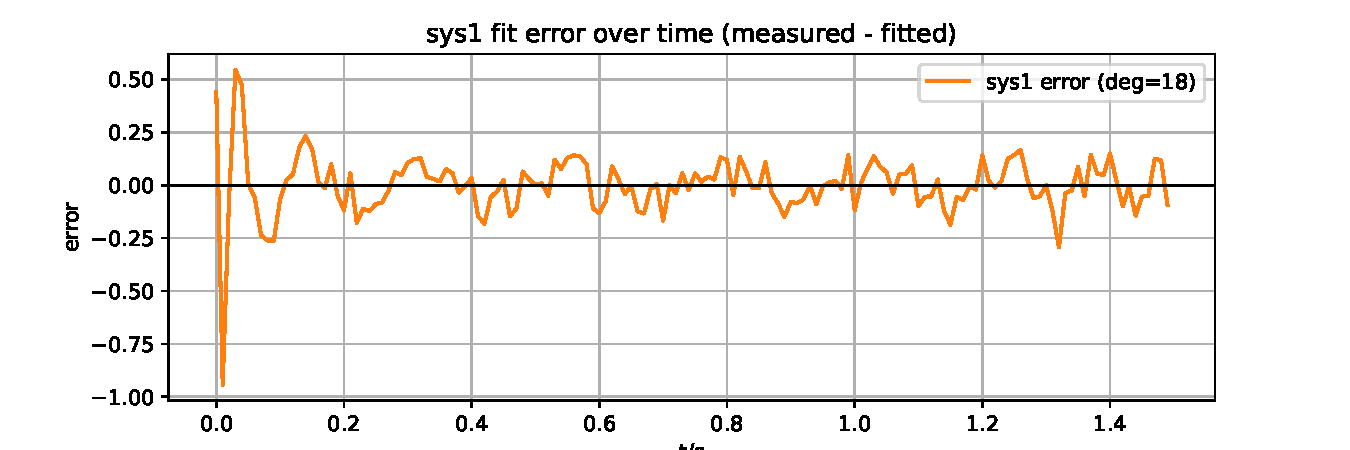
\includegraphics[width=0.8\textwidth]{../02_Preperations/figure_out/sys1_polyfit_error.pdf}
                    \caption[]{}
                \end{figure}


                \subsubsection{Deviations of the System}

        \cleardoublepage

        \section{System 2}\label{sec:system2-it1}
            
            \subsection{Experimentaly Identified system parameters}

                The experimentally identified parameters for the IT1 system are as follows:
                \begin{itemize}
                    \item Proportional gain $K_I$: [add value]
                    \item Proportionalbeiwert $K_p$: [add value]
                    \item Time constant $T_1$: [add value]
                \end{itemize}

            
            \begin{figure}[ht]
                \centering
                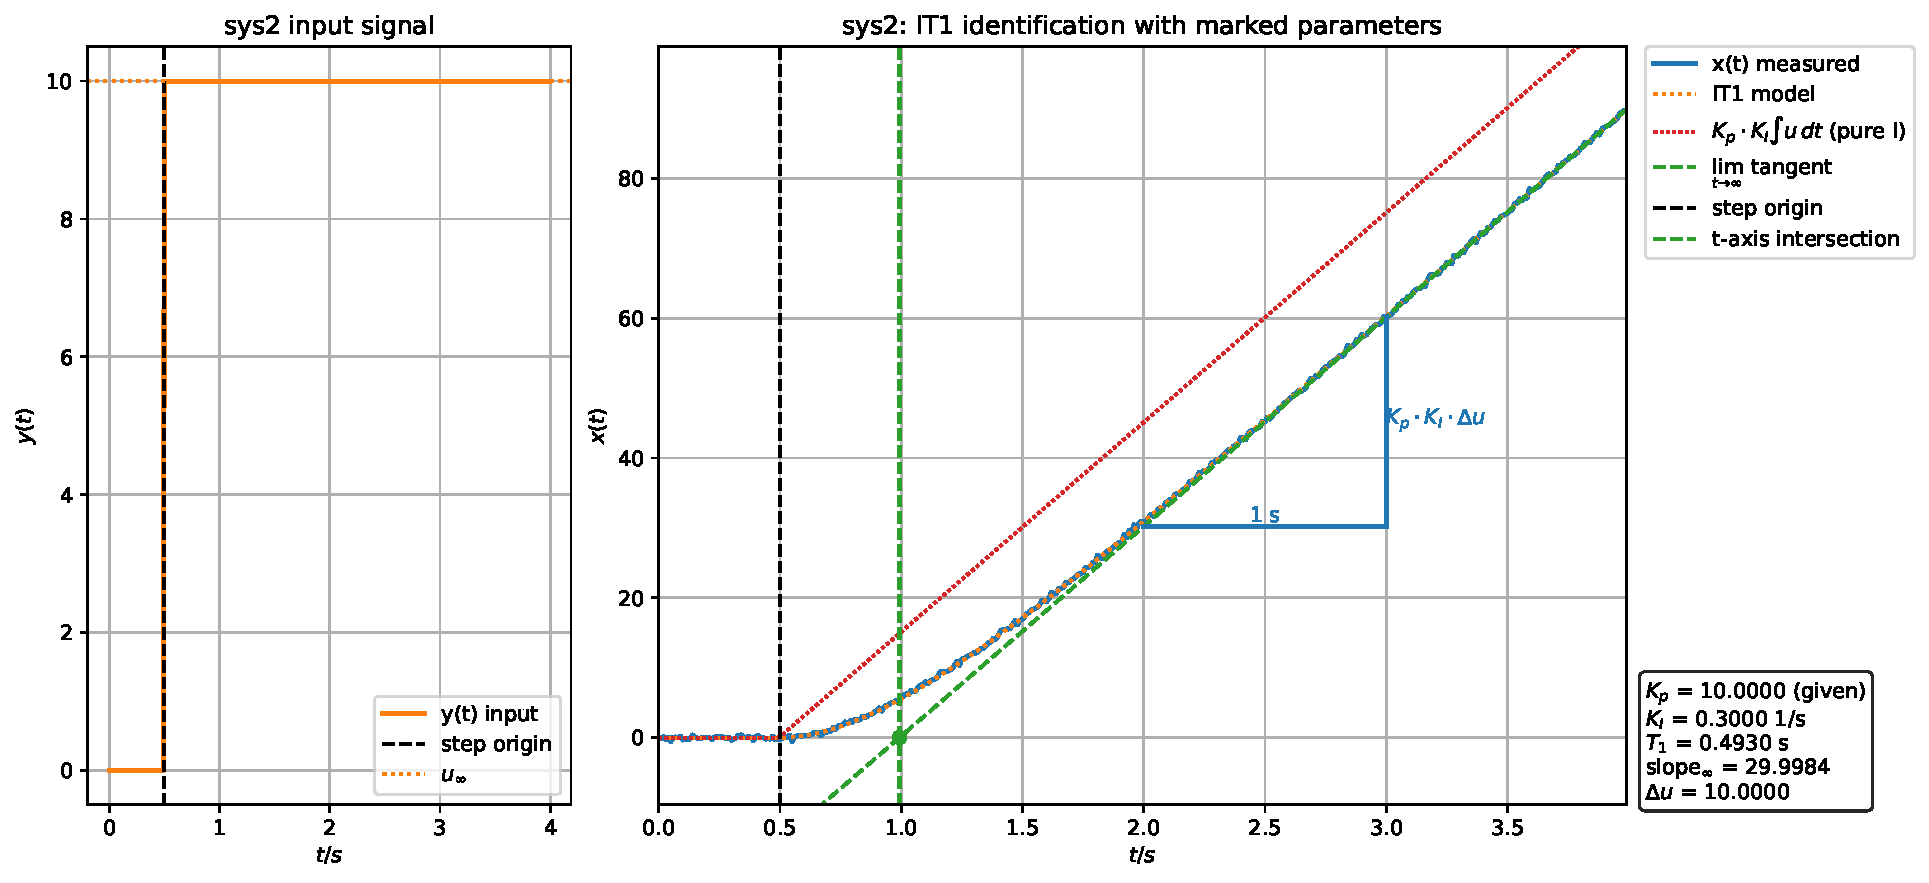
\includegraphics[width=0.8\textwidth]{../02_Preperations/figure_out/sys2_it1_identification.pdf}
                \caption[]{}
            \end{figure}
            
            \todo[inline]{add parameters}

            \subsection{Documentation of the results}

                \subsubsection{Essential Commands}

                \todo[inline]{add essential commands for IT1 identification}

                \subsubsection{Differential Equation}

                \todo[inline]{add differential equation for IT1 system}

                \subsubsection{Transfer Function}

                \todo[inline]{add transfer function for IT1 system}

            \subsection{Realworld Example}

                A clear example of an IT1 element with an upstream dead time is a water tank with a constant inflow and proportional outflow. The inflow corresponds to the input signal, and the water level to the output signal. The storage results in integrative behaviour, whilst the proportional outflow causes first-order damping --- typical of an IT1 system.
                
                In the experimental setup under consideration, a dead-time element was connected upstream of the IT1 element, causing a time delay in the input signal. This means that the system output only reacts to a change after the dead time has elapsed. Such combinations of dead time and IT1 behaviour frequently occur in real-world processes, for example in sluggish piping systems or delayed control variable transmissions.
                description of the respective input and output variables.

            \subsection{Comparison of given System with the response of the identified system}

            \todo[inline]{add short text about differences of the ideal system to the messured IT1 system}
            
            \begin{figure}[ht]
                \centering
                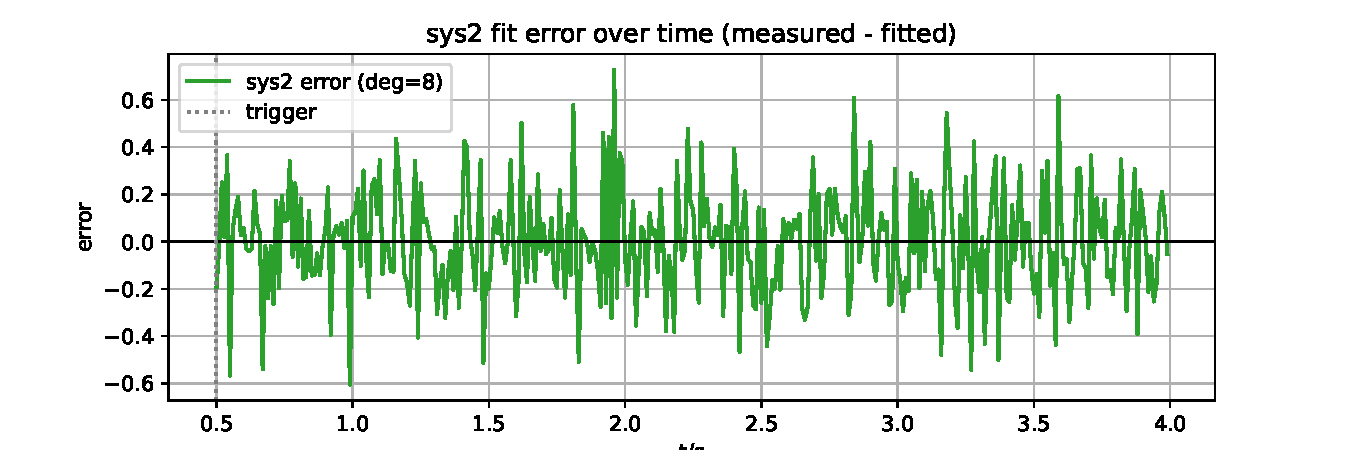
\includegraphics[width=0.8\textwidth]{../02_Preperations/figure_out/sys2_polyfit_error.pdf}
                \caption[]{}
            \end{figure}


                \subsubsection{Deviations of the System}

        \cleardoublepage



    \appendix
        \makeatletter

        
        \chapter{Appendix Frontmatter}
            
            \section{Declerations}

                \todo[inline]{add declerations}

                \cleardoublepage

            \section{List of Figures}

            \listoffigures

            \section{List of Tables}

            \listoftables

            \section{List of Variables and Constants used in this report}

        \chapter{Appendix Code and Resources}

            \section{Code used for the analysis of the Preperations and the Experiment}

            \todo[inline]{add code for the analysis of the preperations, look into jupyter notebook}

            %\lstinputlisting[caption={Code used for the analysis of the Preperations}, label={lst:preperations}]{../02_Preperations/RTP-T2-analysis.ipynb}



        %%%%%%%%%%%%%%%%%%%%%%%%%%%%%%%%%%%%%%%%%%%%%%%%%%%%%%%%%%%%%%%%%%%%%
        \chapter{Bibliography}
        %%%Literaturverzeichnis
        \printbibliography

        %%%%%%%%%%%%%%%%%%%%%%%%%%%%%%%%%%%%%%%%%%%%%%%%%%%%%%%%%%%%%%%%%%%%%

\end{document}